%%%%%%%%%%%%%%%%%%%%%%%%%%%%%%%%%%%%%%%%%%%%%%%%%%%%%
\chapter{Introduction} \label{chap:intro}
\graphicspath{{images/intro/}}
\glsresetall

\ES{Should I frame it as an HRI problem? - alternative: remove first two sentences and update the end}

\gls{hri} explores the challenges of developing robots to interact in human environments and how human beings react to such robots. While not being present in every home yet, robots are quickly propagating through society, for instance as vacuum cleaners, pets, assistants or even friends \citep{belpaeme2012multimodal}. 
To interact in human environments robots require a way to make sense of their sensory inputs and act on the social world; in other words, they need to be sociable \citep{breazeal2004designing}. However, interacting socially with humans is a complex task: the social interaction happens on multiple levels and combines elements from multiple fields \citep{fong2003survey} and social norms used by humans are also transferred to robots \citep{bartneck2004design}. Providing robots with such a complex action policy is a challenge, and will not be solved by programming by hand a static controller covering all the possible aspects and conditions. To interact meaningfully with humans, robots need to learn, constantly expanding and refining their action policy. We propose using the experts in humans interactions, the humans themselves to teach robots to interact socially. By providing control over the robot's actions to a human teacher, robots could learn efficient policies for social interactions from in-situ human supervision. Interactively learning from humans presents a change of paradigm compared to traditional machine learning, as the human has an opportunity to guide the learning, making it more efficient \citep{fails2003interactive,amershi2014power}. Furthermore, by initially framing this work in the context of \gls{hri} we added to the interaction a large set of constraints; consequently a method working in such a complex environment would have applications beyond \gls{hri} e.g. to \gls{ml} and \gls{ai}.

\ES{maybe the reopening is abrupt, might be worth going more in depth about what we have been doing}

%what it is and why it matters and why it is challenging
%
%Robots will inhabit human spaces and need to interact with them in decent ways
%
%Robot behaviour unlikely to be programmable and static
%
%This works explores how robots could interact with humans to learn from them to interact with other humans

%%%%%%%%%%%%%%%%%%%%%%%%%%%%%%%%%%%%%%%%%%%%%%%%%%%%%
\section{Scope}\label{sec:intro-scope}

As shown in \cite{goodrich2007human} only a subset of \gls{hri} is designed to be inherently social. Using Goodrich and Schultz's definition of \gls{hri}, as the study of robots for use by or with humans, an important part of the field does not treat robots as social agents. They are often considered as asocial entities having a task to complete or simply tools to be used by humans. However, as demonstrated by \cite{fincannon2004evidence}, even when used as a teleoperated machines, robots still provoke social reactions and expectations from humans. \cite{fong2003survey} make, among others, the distinction between ``evocative robots'' and ``socially interactive robots''. Evocative robots rely on human tendency to anthropomorphise to succeed in their task, while for ``socially interactive robots'' the social side of the interaction is key. However in \gls{hri}, the sociality of the interaction might not be intended but simply emerge as a by-product of the interaction. As a consequence, in this work we will refer to ``social robots'' as robots interacting in humans environments and considered as ``social agents'' by the humans interacting with them. The intentions of the robot designer or the actual robot's sociality are of minor importance if the humans interacting with the robot project social competencies or expectations on the robot. Regardless on the initial intentions, a robot interacting with humans needs to manage these expectations to ensure the safety and comfort of its human partners. In summary, as soon as a robot interacts with humans, the social side of the interaction needs to be taken into account, the robot needs to be able to interact socially. 

%As described by \cite{goodrich2007human}, \gls{hri} studies ``robotic system for use by or with humans'', consequently, it covers the full spectrum of interactions between humans and robots ranging from physical assistance and teleoperation to social companions. In \cite{fong2003survey}, authors refer to ``socially interactive robots'', as ``robot for which social interaction plays a key role''. As such, these socially interactive robots exclude robot interacting purely physically with humans, such as exoskeleton, physical rehabilitation or pure teleoperation as in robotic assisted surgery. However, even with robots not intended to behave socially, humans might create bonds and relationships \cite{fincannon2004evidence}. As such, this review extends the concept of ``socially interactive robots'' not only to robots designed to interact socially, but to robots eliciting social response from the hu

%if a robot is consider as a social agent, it needs to be able to interact socially

%social robots = robots perceived as social agents in human environments.

Enabling a robot to interact socially with humans is a complex task. The robot needs to make sense a large input space, from low level sensory feedback (e.g. joint angles or camera pixels) to high level concepts (e.g. hand-coded events or learned features). And based on the interpretation of these inputs and rules defining a behaviour, the robot needs to select an action or a plan to achieve an assigned goal. As this task covers most of the areas of robotics \citep{fong2003survey}, this section will precise the scope of the research conducted in this thesis.

\subsection{Frame}

The context of the research conducted here is finding a way for robots to interact efficiently with humans. It has been argued by many researchers  \citep{dautenhahn2004robots,billard2008robot} that robots need to adapt to their users and be able to learn from them. Social robots cannot apply a one-size-fits-all policy programmed in advance by engineers and suited to every possible interaction partners. Robots need the capability to learn an interactive behaviour, improving their skills as they interact in the world and personalising their policy to their users; and enabling such a learning is focus of this thesis.

Throughout this thesis we make the assumption that a human knows how the robot should interact. A person, generally not the engineers initially developing the robot, possesses some expertise which should be transferred to a robot. This expertise is not related to theoretical knowledge in \gls{ml}, robotics or other scientific fields but defines how the robot should behave. For instance,  it could take the form of the steps of a therapy a robot should deliver to the child (known by a therapist) or more simply a senior's preferences and desires concerning a robot companion's behaviour. As a consequence, robot users should be able to teach their robot, to transfer their knowledge to their robot without requiring technical expertise.

Although the ultimate goal of this research is to explore how robots could learn to interact socially and efficiently with humans; by making the assumption that the interactive knowledge should be provided by a human, the resulting question of this thesis is: \emph{How humans could teach robot to interact?}. As such, this research work aims to provide a convenient and efficient way for domain experts to inculcate robots with their interactive knowledge. In other words, this research explores the requirements on an interaction frameworks allowing humans to teach robot to interact socially in human environments and the impacts such a framework would have on the interaction.

%\subsection{Environment} 
\subsection{Type of Interactions}

By focusing the research on using humans to teach robots, we add a second human-robot interaction to the application interaction: the interaction between the robot and the teacher. This results in two intertwined human-robot interactions: the application interaction, between the application target and the robot and the teaching interaction, between the teacher and the robot (cf. Figure \ref{fig:intro_setup}). And the end goal of teaching interaction is to achieve high standards in the application interaction. This results in a general triadic interaction between a human target, a robot and a human teacher. 

\begin{figure}[ht]
	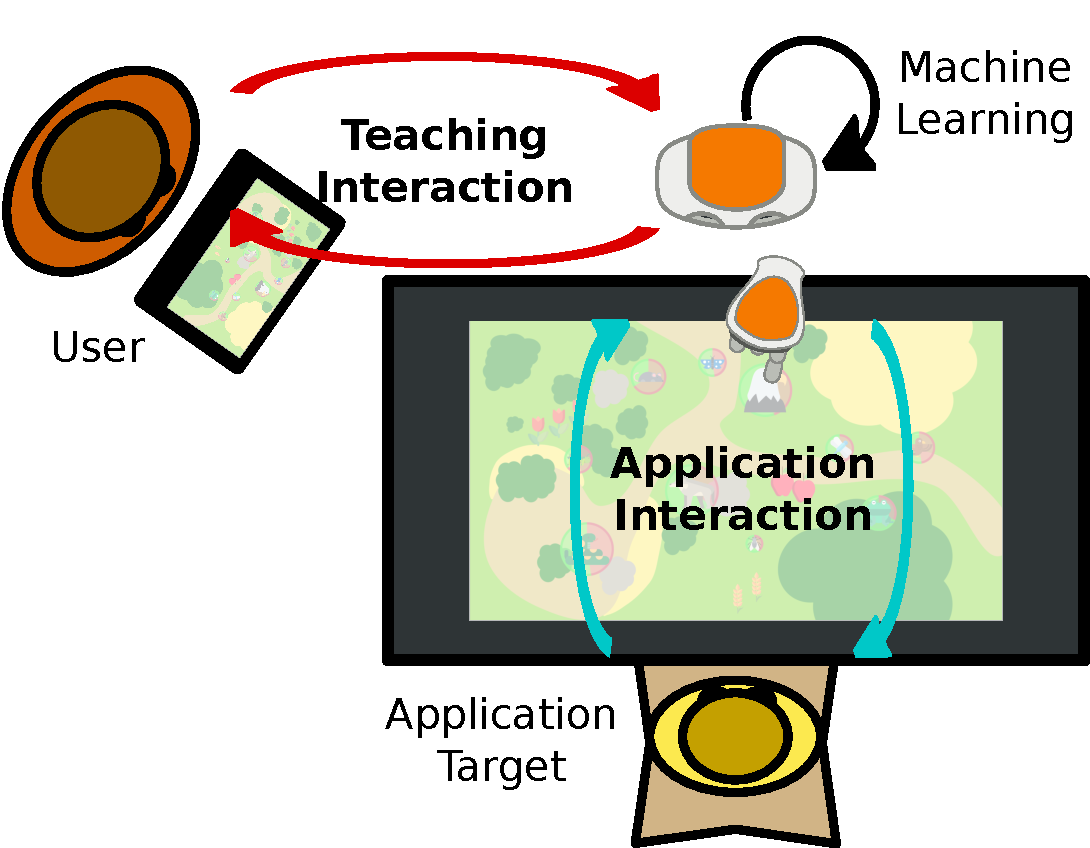
\includegraphics[width=.7\linewidth]{setup.pdf}
	\centering
	\caption{The typical interaction used in this research: a robot interacts with a target in an application interaction and learns from a domain expert through a teaching interaction.}
	\label{fig:intro_setup}
\end{figure}

While having been pursued by considering mostly \gls{hri} as an application interaction, the work presented in this thesis is applicable to teaching a robot, or more generally agents, many type of interactions, not only with humans. Indeed, interacting with a human is a high stake scenario, where misbehaving can be costly, where datapoints for learning can be tedious to acquire and with a high diversity between different partners. Other types of interaction could be less constrained, complex or with lower stakes. Consequently, by addressing a challenging task (teaching a robot to interact socially with humans), this approach is also be suited to a wide range of other tasks (such as manipulation, classification or navigation). In the more general case, a user has a task they would like an artificial agent to complete and they can teach it. Through the teaching interaction, the human can supervise the agent, demonstrating it what it should do and teaching it an efficient action policy in the application interaction with the target. 

%The application target could be another human (such as a child receiving teaching support from the robot) or just parts of the environment if the robot has to complete a manipulation of navigation task (such as picking up a book in the library).

%Mention more the social side of the interaction??

%Robots considered in this thesis evolve in human-centred environments and are expected to provide some support to the surrounding humans and achieve a specific goal assigned to them. Human interactions and by extend human environments are in essence social, they are governed by social norms, and on the adhesion to these norms depends the success of the interaction. 

%%%%%%%%%%%%%%%%%%%%%%%%%%%%%%%%%%%%%%%%%%%%%%%%%%%%%
\section{The Thesis}\label{sec:intro-thesis}
\ES{rephrase}
The main thesis this document seeks to put forward is as below.
\begin{quote}
	\textbf{A robot can learn to interact meaningfully with humans in an efficient and safe way by receiving supervision from a human teacher in control of the robot's behaviour.}
	%This supervision will lead to an efficient, safe and low human-workload teaching and autonomous behaviour.	
\end{quote}

\ES{rephrase}
Additional research questions are also introduced here. These research questions are used to support and direct the experimental research conducted in pursuit of demonstrating the primary thesis.

\begin{itemize}
	\item [RQ1] \emph{What are the requirements of a robot controller to ensure a behaviour suited to \gls{hri}?} 
	
		By interacting with humans, robots enter the social world and have to conform to human expectations while ensuring they can reach their goal. This research question studies which constraints interacting in the human world put on the robot's controller. 
		
    \item [RQ2] \emph{What interaction framework would allow a human to teach a robot while validating the requirements from RQ1?}
    
    	%While RQ1 provides requirements for a robot controller, the task of designing a interaction framework allowing a human to teach remains. 
    	This research question address what principles of interaction could lead to an efficient teaching interaction between a robot and a human whilst validating the requirements from RQ1. 
    	
    \item [RQ3] \emph{Could a robot decrease its supervisor's workload by learning from their supervision?}
    
        Controlling a robot is a significant workload for the human supervisor. This question explores if including a learning component in the robot behaviour could alleviate the human workload by taking over some of the mental and physical requirements of the robot control. Additionally, this question explores if this learning impacts the performance in the task.
%        \gls{woz} is an approach widely used in \gls{hri} \citep{riek2012wizard}, whereby a human teleoperates a robot to have it interact with other humans. However, this method applies a high workload on the operator and is not scalable. Using \gls{ml} to learn from this operator online might decrease the operator's workload without decreasing the quality of the robot behaviour.
    
    \item [RQ4] \emph{How providing the teacher with control over the learner's actions impacts the teaching process?} 
    
    	Teaching robots has a unique property compared to teaching humans in the fact that the teacher could have total control over the learner's actions. This question explores if this control could lead to a faster and a more efficient learning while lightening the process for the teacher.
	%    In the context of \gls{iml}, a human can provide inputs to an agent to speed up the learning. Other \gls{iml} \citep{thomaz2008teachable,knox2009interactively} focus on feedback from the human with limited or no control over the agent's actions. However, increasing the control should speed up the learning and reduce the number of errors made by the robot.

	\item [RQ5] \emph{How teaching a robot to interact socially impacts the two humans involved in the overall triadic interaction?}
%		How an interaction framework validating the requirements from RQ1 impact humans interacting with a robot when it is learning?}
	
		%RQ2 explores how a teaching framework could in theory validate the requirements from RQ1. 
		When using humans to teach robots, two interactions are linked, this questions studies if this teaching could happen while validating the requirements from RQ1 and the potential impact of this coupling of interactions on the teaching process.
		%This research question evaluates if the framework proposed by exploring RQ2 would satisfy the requirements from RQ1 during the teaching process. 
		%Talk about impacts on both humans?
		
    \item [RQ6] \emph{After receiving supervision from a human, could a robot behave autonomously in a social context?}
%    \item [RQ5] \textbf{How can a human teach a robot to interact with other humans?} %???

	 	After having been taught, a robot can be deployed to interact autonomously in the real world. This questions analyses the robot's behaviour when interacting autonomously and explores the efficiency of a teaching in situ in providing the robot an autonomous behaviour validating principles from RQ1.
	 	%\gls{sparc} has been designed to allow non-experts in \gls{ml} to teach agents how to interact during the interaction. Human-robot interactions provide a perfect test for this approach: using a human to teach a robot how to behave in this complex and non-deterministic environment.
	 
\end{itemize}

%%%%%%%%%%%%%%%%%%%%%%%%%%%%%%%%%%%%%%%%%%%%%%%%%%%%%
\section{Approach and Experimentation}

\subsection{New Teaching Framework}
\ES{improve}
To address the requirement on a robot controller emerging by addressing RQ1, in this work, we propose the \gls{sparc}, a novel teaching framework intended to provide a way for non-experts in robotics to safely teach a robot to interact with humans. This research work describes and justifies this approach and evaluates its impact though three studies.

\subsection{Study Design} 

To address the main thesis of this work and RQ3 to RQ6, we designed and ran three studies, each of which is described in depth in a chapter. These studies evaluate the impacts of \gls{sparc} on different parts of the teaching and application interactions. The two first studies focused on how humans could teach robots, and consequently required repeatable environments to compare humans' efficiency and experiences when teaching a robot. The last study was run in a school with a single human teaching a robot to interact with children over multiple sessions and explored if \gls{sparc} could be used to teach a robot to interact with humans. All the studies used \gls{sparc} in the type of interaction presented in Figure \ref{fig:intro_setup}, i.e. a teacher wants a robot to complete a task (included but not limited to human interaction) and can control the robot's actions through an interface. 

The first study (Chapter \ref{chap:woz}) explored if \gls{sparc} could be used to provide learning to a robot in a \gls{woz} interaction and if this learning impacts the workload and performance of the teacher in the task. We took inspiration of \gls{rat} and decided to replace the child interacting with the wizarded-robot by a second robot running a model of a child and presenting typical features observed in children (such as probabilistic behaviour, partial observability of state and absence of easily definable optimal action policy). This repeatable environment allowed us to evaluate in a controlled study the impact of \gls{sparc} on the teacher.

The second study (Chapter \ref{chap:control}) compared \gls{sparc} to an other method in \gls{iml}: \gls{irl} in a replication of the virtual environment initially used to test \gls{irl}. The main difference between the two methods resides in the quantity of control provided to the teacher; unlike \gls{irl}, \gls{sparc} provides teachers with full control over the robot's actions. In this study, participants controlled a virtual robot on a computer and had to teach it how to solve a task.

Finally, the last study (Chapter \ref{chap:tutoring}) deployed \gls{sparc} in a real interaction with humans, to teach children about food chains. This study used exactly the paradigm described in Figure \ref{fig:intro_setup}: a child interacting with a robot and a teacher using a tablet to control the robot's actions and teaching the robot how to interact efficiently with children.

%%%%%%%%%%%%%%%%%%%%%%%%%%%%%%%%%%%%%%%%%%%%%%%%%%%%%
%\section{Key Concepts and Terminology}\label{sec:intro-concepts}
%
%\subsection{Terminology}
%
%Not sure if worth including
%
%Throughout this thesis, the terms `wizard', `supervisor', `user', `expert' and `teacher' have been used interchangeably to represent the people in control of a robot's action and teaching that robot an action policy.
%
%agent and robot
%
%\begin{itemize}
%	\item \textbf{Appropriateness}:
%	\item \textbf{Adaptivity}
%	\item \textbf{Autonomy}
%	\item \textbf{Supervised Autonomy}
%	\item \textbf{Learning}
%	\item \textbf{Teacher, wizard, user, expert and supervisor}
%	\item \textbf{Robot, agent and learner}
%\end{itemize}

\subsection{Learning Algorithms}
\ES{put NN in gls - fix capital letter}
To enable robots to learn from humans, they need to be equipped with \acrfull{ml}, i.e. an algorithm statistically learning a mapping between inputs and outputs. Two main categories of \gls{ml} are relevant this research: \gls{sl} and \gls{rl}.

\ES{reorganise}
\gls{sl} aims to learn a mapping between inputs and outputs to automatically reproduce a desired known behaviour. It uses a dataset of labelled example and optimises an algorithm to minimise the prediction error of labels \citep{russell2016artificial}. This aim, reproducing a desired behaviour, is especially connected with the work carried out in this research. By learning to reproduce the teacher's policy, the robot should reach an efficient behaviour in the target application. Typical examples of \gls{sl} used in this study are \gls{ann} and nearest neighbours methods. \gls{ann} model loosely the way brains and neurons work by having a group of interconnected `neurons'. By changing the connections between the neurons, the network learns to reproduce the desired values on the output nodes according to the inputs. On the other hand, nearest neighbours methods are instance based methods, they compare the distance in a feature space between a point to classify and the different instances stored in a dataset and select the value of a majority of nearest neighbours in that space.

Unlike \gls{sl} which reproduces a known behaviours, \gls{rl} aims at providing an agent with the capacity to discover the world it interact in and learn from this interaction with the world \citep{sutton1998reinforcement}. The agent has access to a description of the state and actions it can do, and depending of the action selected, the state will change and the agent will receive a reward. The goal of the agent is to find an optimal policy maximising a notion of cumulated reward. \gls{rl} is also linked to the work presented in this thesis: by allowing robots to learn to interact in human environments, we would reach our goals of efficient human-robot interactions.

Due to the relevance of both fields to this research (enabling humans to teach robots to interact), algorithms from both categories have been used. The first study presented in Chapter \ref{chap:woz} used a feed forward neural network learning to reproduce a teacher policy. The second study in Chapter \ref{chap:control} used \gls{rl} to combine human guidance and environmental and human rewards to learn an efficient action policy. The last study presented in Chapter \ref{chap:tutoring} used an instance based algorithm adapted from Nearest Neighbours to enable online quick and efficient learning. More details about each algorithms and their related work can be found in the associated chapters.

\subsection{Data Analysis}
Graphs presented throughout this thesis have been generated using the seaborn package for Python and matplotlib \cite{waskom2017seaborn}. Often, we used violin plots, a graphical representation featuring the kernel density estimation of the distribution potentially producing the data. Statistical analysis in Chapters \ref{chap:control} and \ref{chap:tutoring} have been made using the Jasp software \cite{jasp2018}. Jasp offers a Bayesian counterpart to classic statistical test, making them more robust and allowing to observe the presence or absence of effect. As such, instead of a $p-value$, the Bayes factor $B$ is reported and represents how much of the variance on the metric is explained by a parameter (if $B < 1/3$ there is no impact, if $B > 3$ the impact is strong, and if $1/3<B<3$ the results are inconclusive; \citealt{jeffreys1998theory,dienes2011bayesian}). 

\subsection{Terminology}

Throughout this thesis, the terms `wizard', `supervisor', `user', `expert' and `teacher' have been used interchangeably to represent the people in control of a robot's action and teaching that robot an action policy. Similarly, we refers to the robot as `robot', `agent' or `learner' depending of the situation.
%%%%%%%%%%%%%%%%%%%%%%%%%%%%%%%%%%%%%%%%%%%%%%%%%%%%%
%\section{Challenges}
%
%Complexity of interactions with humans: complex world, safety, workload and so on
%
%not sure if needed?

%%%%%%%%%%%%%%%%%%%%%%%%%%%%%%%%%%%%%%%%%%%%%%%%%%%%%
\section{Contributions}\label{sec:intro-contr}

This research work contributed both scientifically (by creating and evaluating \gls{sparc}) and technically (by developing software to multiple projects) to the state of the art in \gls{hri} and especially in teaching robots to interact with humans. This section highlights the original contribution of this thesis and indicates the relevant chapters and published work.

\subsection{Scientific Contributions}
\begin{itemize}
	\item Design of \gls{sparc}, a new interaction framework for teaching agents in a safe way. (Chapter \ref{chap:sparc}; \citealt{senft2015human,senft2015sparc})
	\item Evaluation of \gls{sparc} in three studies. (Chapters \ref{chap:woz}, \ref{chap:control} and \ref{chap:tutoring})
	\item Demonstration of the importance of control over the robot's action when teaching a robot to interact. (Chapter \ref{chap:control}; \citealt{senft2016sparc,senft2017supervised})
	\item Design of a lightweight algorithm to quickly learn from demonstration in complex environments. (Chapter \ref{chap:tutoring}; \citealt{senft2017toward})
	\item Application of \gls{iml} to safely teach robots social autonomy from in situ human supervision. (Chapter \ref{chap:tutoring}; \citealt{senft2018robots})
\end{itemize}

\subsection{Technical Contributions}
\begin{itemize}
%	\item Development of three different studies to evaluate \gls{sparc} in three different scenarios (supervised robot-robot interaction, virtual robot and real word \gls{hri}).
	\item Partial development of a cognitive architecture and two tools for the \acrshort{dream} project (European FP7 project: 611391). \citep{esteban2017build}
	\item Development of an autonomous robot controller to support cardiac rehabilitation in the Human-Robot Interaction Strategies for Rehabilitation based on Socially Assistive Robotics project (Royal Academy of Engineering: IAPP\textbackslash1516\textbackslash137). \citep{lara2017human,casas2018social}
	\item Development of a wizard interface for the Freeplay-Sandbox\footnote{\url{https://github.com/freeplay-sandbox}}. \citep{lemaignan2017free}
\end{itemize}
	
%%%%%%%%%%%%%%%%%%%%%%%%%%%%%%%%%%%%%%%%%%%%%%%%%%%%%
\section{Structure}\label{sec:intro-struct}
\ES{Rephrase}
The structure of this thesis is outlined below to provide an overview of the content and context for each chapter. A summary of key experimental findings are included at the start of each relevant chapter for ease of reference. 

\begin{itemize}
	%From James, could probably be updated
	\item This chapter provided an introduction to the general field of this research (robots learning to interact with and from humans), the research questions including the central \emph{thesis}, the scope and the contributions of the work presented in later chapters.  

	\item Chapter~\ref{chap:background} provides a description of the different fields of social \gls{hri} and draws requirements for controllers of robots interacting with humans. In a second part, it analyses the current robot controllers used in \gls{hri} identifying that no current controller fits these requirements. Finally, it introduces \gls{iml} and proposes to apply it to \gls{hri} as a way to validate the previously defined requirements.
	
	\item Chapter~\ref{chap:sparc} proposes a new interaction framework, \gls{sparc}, as a way to apply \gls{iml} to \gls{hri} while validating the three requirements proposed in Chapter \ref{chap:background}. This chapter describes the principles behind \gls{sparc} and the expectations and limits this method could have.
	
	\item Chapter~\ref{chap:woz} presents results from a first study evaluating the impact of \gls{sparc} on the supervisor's workload and performance compared to \gls{woz}. Results support the hypotheses, validating some of the motivations of \gls{sparc} (a learning robot would reduce the workload on a supervisor).
	
	\item Chapter~\ref{chap:control} presents results from a second study comparing \gls{sparc} to \gls{irl}, another interaction framework from \gls{iml}. The main difference between the two approaches lies in the amount of control the teacher has: with \gls{sparc}, the teacher can correct any action executed by the robot. Results from a 40 participants study support that this control improves the efficiency of the learning (improving the performance, reducing the time and the number of inputs required to teach as well as decreasing the risks taken during the teaching phase).
	
	\item Chapter~\ref{chap:tutoring} presents the first study where \gls{sparc} has been applied to a real world \gls{hri}, child tutoring. Results demonstrate that, while not impacting the learning gain of the session, a supervised robot elicit richer child behaviour compared to a passive robot. Furthermore, by learning using \gls{sparc} an autonomous robot can reach policy similar to the teacher's one and achieve the same impact on the children. These results support \gls{sparc} as a teaching method allowing to transfer a social and technical action policy from human to a robot in a safe way and leading to efficient autonomous behaviour.
	
	\item Chapter~\ref{chap:discussion} presents a discussion from the main findings from the previous chapters and presents limitations and future directions of research for \gls{sparc}.
	
	\item Chapter~\ref{chap:conclusion} concludes the thesis and presents a summary of the main contributions.
	
\end{itemize}
